\chapter{Strumenti}
In questo capitolo si descrivono gli strumenti usati per lo sviluppo del progetto: 
\begin{itemize}
    \item \textbf{Processore Microblaze}, il processore MicroBlaze è stato utilizzato come base per l'implementazione dell'interprete e del suo relativo set di istruzioni (sezione \ref{Microblaze}).
    \item \textbf{Scheda Alveo U50}, un'FPGA di Xilinx, è stata utilizzata per condurre gli esperimenti di implementazione  (sezione \ref{Alveo}).
    \item  \textbf{Software Vitis}, fondamentale per programmare e sfruttare al massimo le capacità della scheda U50  (sezione \ref{Vitis}).
    \item \textbf{Il framework OpenCL} è stato impiegato per consentire la comunicazione tra l'host e l'FPGA, sfruttando al meglio le capacità di accelerazione hardware (sezione \ref{Opencl}).
    \item \textbf{Linguaggio di programmazione C++/C}, il linguaggio di programmazione C++ è stato utilizzato per gestire le chiamate OpenCL e altre parti dell'applicazione. Inoltre, il linguaggio C è stato impiegato per scrivere l'interprete stesso . (sezione \ref{C++/C})
\end{itemize}

\clearpage 

\section{Microblaze}
%\begin{figure}[h!]
%    \centering
%    
\includegraphics[scale=0.4]{images/Capitolo2/1_im.png} 
%    \caption{Logo}
%    \label{microb}
%\end{figure}

\label{Microblaze}
Il MicroBlaze è un processore a microcontrollore configurabile (soft core) progettato da Xilinx, un'azienda specializzata in dispositivi programmabili come FPGA (Field-Programmable Gate Arrays) e SoC (System on Chip).

E' stato sviluppato per essere implementato all'interno delle schede FPGA Xilinx e svolge il ruolo di un processore personalizzabile, ovvero che può essere configurato in base alle specifiche esigenze dell'applicazione.

\vspace{0,5cm}

Alcune caratteristiche possono essere riassunte come segue:  

\begin{enumerate}
    \item \textbf{Configurabilità/Flessibilità.} Gli sviluppatori possono scegliere tra le varie versioni del Softcore e selezionare le funzionalità richieste per l'applicazione specifica che cercano di sviluppare, come la cache, le varie interfacce per le periferiche, l'unita di gestione degli interrupt e altro. Questo rende il processore utilizzabile in una varietà di applicazioni, tra cui controllo industriale, comunicazioni, video, sistemi embedded, e molto altro.
    \item \textbf{Set di istruzioni.} Il MicroBlaze utilizza un set di istruzioni RISC (Reduced Instruction Set Computer) e può essere personalizzato per includere istruzioni personalizzate o estensioni per ottimizzare l'elaborazione specifica dell'applicazione.
    \item \textbf{Consumo energetico.} Il MicroBlaze è stato progettato per essere efficiente dal punto di vista energetico, il che lo rende adatto per dispositivi a batteria e sistemi embedded in cui il consumo energetico è un aspetto critico.
    \item \textbf{Supporto software.} Xilinx fornisce un ambiente di sviluppo software, come Xilinx SDK (Software Development Kit), che semplifica la programmazione e il debug di applicazioni.
\end{enumerate}

\vspace{0,5cm}

In sostanza, il MicroBlaze è un processore personalizzabile che può essere adattato per adempiere a una vasta gamma di esigenze, ed è reso più facile da utilizzare grazie al supporto software fornito da Xilinx.

All'interno di questa tesi, abbiamo utilizzato solo una piccola parte delle istruzioni di questo processore. Abbiamo scelto di non considerare le sue caratteristiche hardware in quanto non erano necessarie per dimostrare la fattibilità di questa implementazione su un dispositivo FPGA.

\clearpage 

\section{Alveo U50}
\label{Alveo}

\vspace{0,3cm}


La Alveo U50 è una scheda di accelerazione FPGA sviluppata da Xilinx, è stata creata per consentire l'implementazione di software personalizzato che può essere accelerato tramite hardware. Questa combinazione offre efficienza e velocità che non sono raggiungibili attraverso il normale metodo di programmazione della CPU che ospita l'acceleratore. 

\begin{figure}[h!]
    \centering
    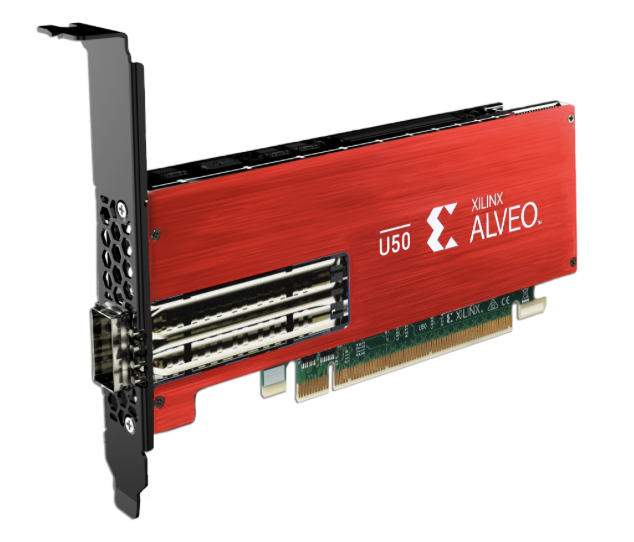
\includegraphics[scale=0.4]{images/Capitolo2/2_im.png} 
    \caption{Alveo U50}
    \label{U50}
\end{figure}

In altre parole, la Alveo U50 fornisce la capacità di adattare e ottimizzare il software per ottenere prestazioni eccezionali grazie all'elaborazione hardware su FPGA.

La Alveo U50 è caratterizzata da una buona potenza di calcolo e un'architettura molto configurabile, il che la rende adatta per una varietà di settori, tra cui intelligenza artificiale, elaborazione di dati, e molto altro. Inoltre, questa scheda è progettata per ridurre al minimo il consumo energetico, il che la rende ideale per applicazioni che richiedono una gestione efficiente delle risorse.

\vspace{0,3cm}

\begin{figure}[h!]
    \centering
    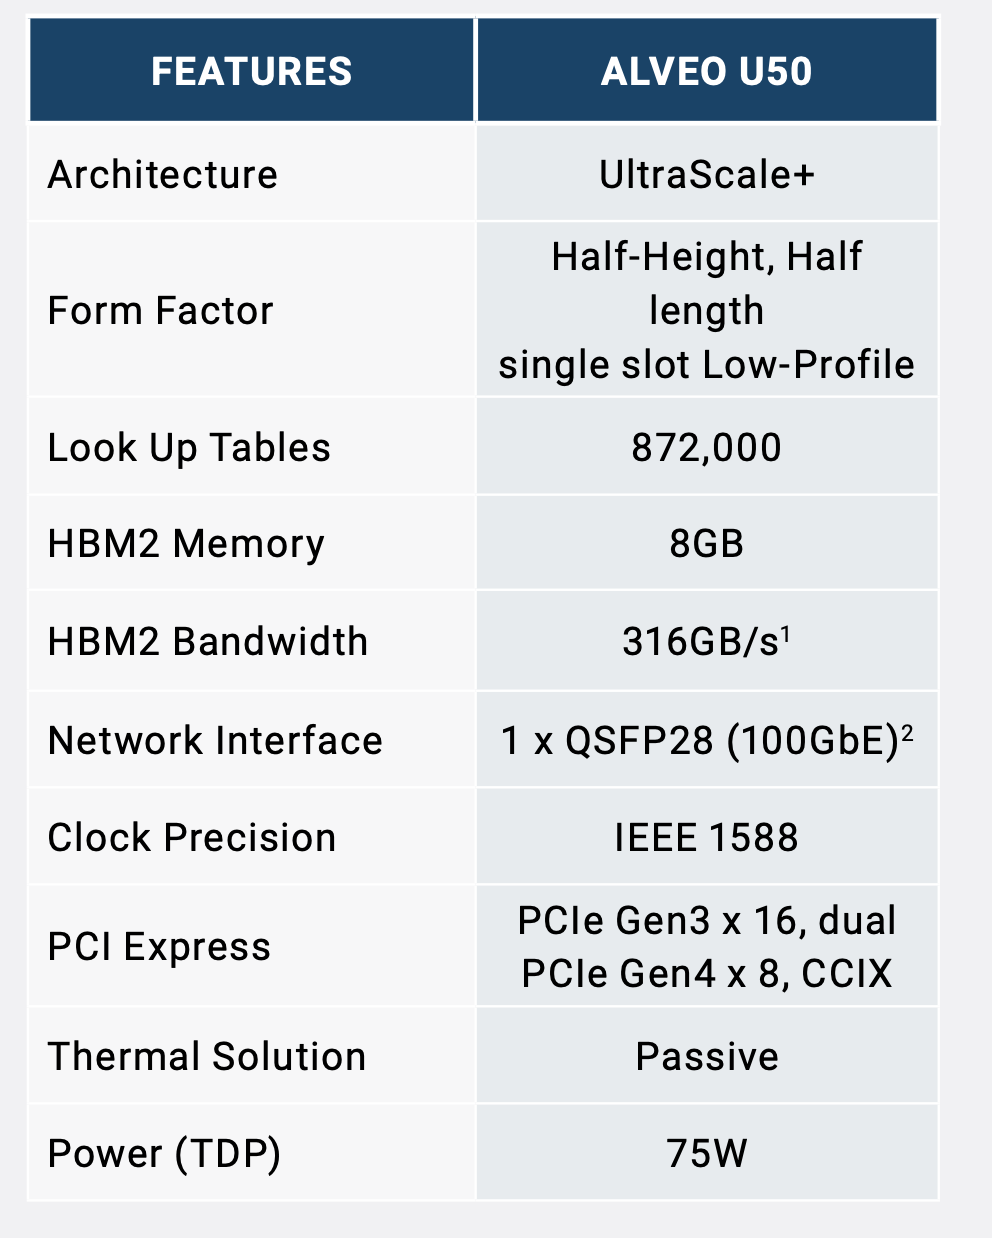
\includegraphics[scale=0.3]{images/Capitolo2/3_im.png}
    \caption{Specifiche Alveo U50 \cite{sitoAlveoU50}}
    \label{Specifiche-U50}
\end{figure}

Nella Tabella \ref{Specifiche-U50} si trovano riassunte le principali caratteristiche e "dimensioni della scheda.
Abbiamo scelto questa scheda perché era quella a disposizione nella macchina host usata per gli esperimenti di implementazione.
\vspace{0,3cm}

\section{Vitis}
\label{Vitis}
Come scritto nella documentazione:

\vspace{0,2cm}

"The AMD Vitis™ software platform is a development environment for developing designs that includes FPGA fabric, Arm® processor subsystems, and AI Engines" \cite{sitoAMDvitis}. 

\vspace{0.4cm}

\noindent In particolare Vitis Software Platform mette a disposizione i seguenti tool:

\begin{enumerate}
    \item \textbf{Vitis Embedded} – per scrivere applicazioni in C/C++ e farle eseguire in codice per processori arm su piattaforme embedded.
    \item \textbf{Compiler and simulators} – per implementare applicazioni usando l'AI Engine array.
    \item \textbf{Vitis HLS} – per scrivere applicazioni C/C++ basate su gli IP blocks che hanno come target di esecuzione le schede FPGA.
    \item \textbf{Vitis Model Composer} – "A model-based design tool that enables rapid design exploration within the MathWorks Simulink® environment"\cite{sitoAMDvitis}.
    \item Un set di funzioni opensource tipo  DSP, Vision, Solver, Ultrasound, BLAS, e altre ancora, che possono essere utilizzate nelle FPGA o con gli AI Engines in applicazioni "custom" .
\end{enumerate}

\vspace{0.3cm}
\noindent Contrariamente all'approccio tradizionale RTL (Register-Transfer Level) di progettazione hardware, Vitis utilizza HLS (High-Level Synthesis), che rappresenta un cambiamento radicale di paradigma  nella progettazione di FPGA.

\vspace{0.3cm}

\noindent Questo perché l'approccio HLS permette di scrivere applicazioni utilizzando codice in linguaggi di alto livello come C, C++, o OpenCL, invece di descrivere esplicitamente la logica hardware, cosi da tradurre il codice in un circuito hardware eseguibile dalla FPGA senza una vera e propria programmazione dettagliata di RTL.

\vspace{0.3cm}

\noindent Questo approccio rende accessibile la potenza di elaborazioni di un FPGA a sviluppatori che non hanno una profonda conoscenza del linguaggio RTL, cosi anche da rendere più semplice lo sviluppo di applicazioni in settori come l'intelligenza artificiale, elaborazione di immagini, e altro ancora.

\clearpage 

\section{OpenCL}
\label{Opencl}

"OpenCL™ (Open Computing Language) is an open, royalty-free standard for cross-platform, parallel programming of diverse accelerators found in supercomputers, cloud servers, personal computers, mobile devices and embedded platforms." \cite{sitoOpencl}

\begin{figure}[h!]
    \centering
    
\includegraphics[scale=0.2]{images/Capitolo2/4_im.png}
    \caption{OpenCL logo}
    \label{Specifiche-U50}
\end{figure}

Il framework messo a disposizione da OpenCL crea uno standard per lo sviluppo di applicazioni parallele che richiedono di sfruttare a pieno la potenza dei calcolatori presenti al giorno di oggi, i quali sono molto eterogenei.

\vspace{0,3cm}

OpenCL velocizza l'esecuzione delle applicazioni eseguendo il codice più dispendioso dal punto di vista computazionale in acceleratori, in questa maniera gli sviluppatori possono scrivere dei kernel in C/C++, che saranno caricati tramite un device compiler per l'esecuzione parallela sui dispositivi di accelerazione.

\vspace{0,3cm}
\vspace{0,3cm}

\noindent Un applicazione OpenCL è divisa in due parti: 
\begin{itemize}
    \item \textbf{host:} questa parte è scritta in un un linguaggio come C o C++, e compilata con i compilatori tradizionali per essere eseguita sulla CPU del calcolatore host.
    \item \textbf{device:} è la parte che può essere compilata "on the fly" (ovvero tramite l'utilizzo di chiamate speciali dell'API a tempo di esecuzione), oppure si può compilare prima che l'applicazione vada in esecuzione cosi da rendere portabile il binario generato in una rappresentazione intermedia chiamata SPIR-V di Khronos. 
\end{itemize}

\begin{figure}[h!]
    \centering
    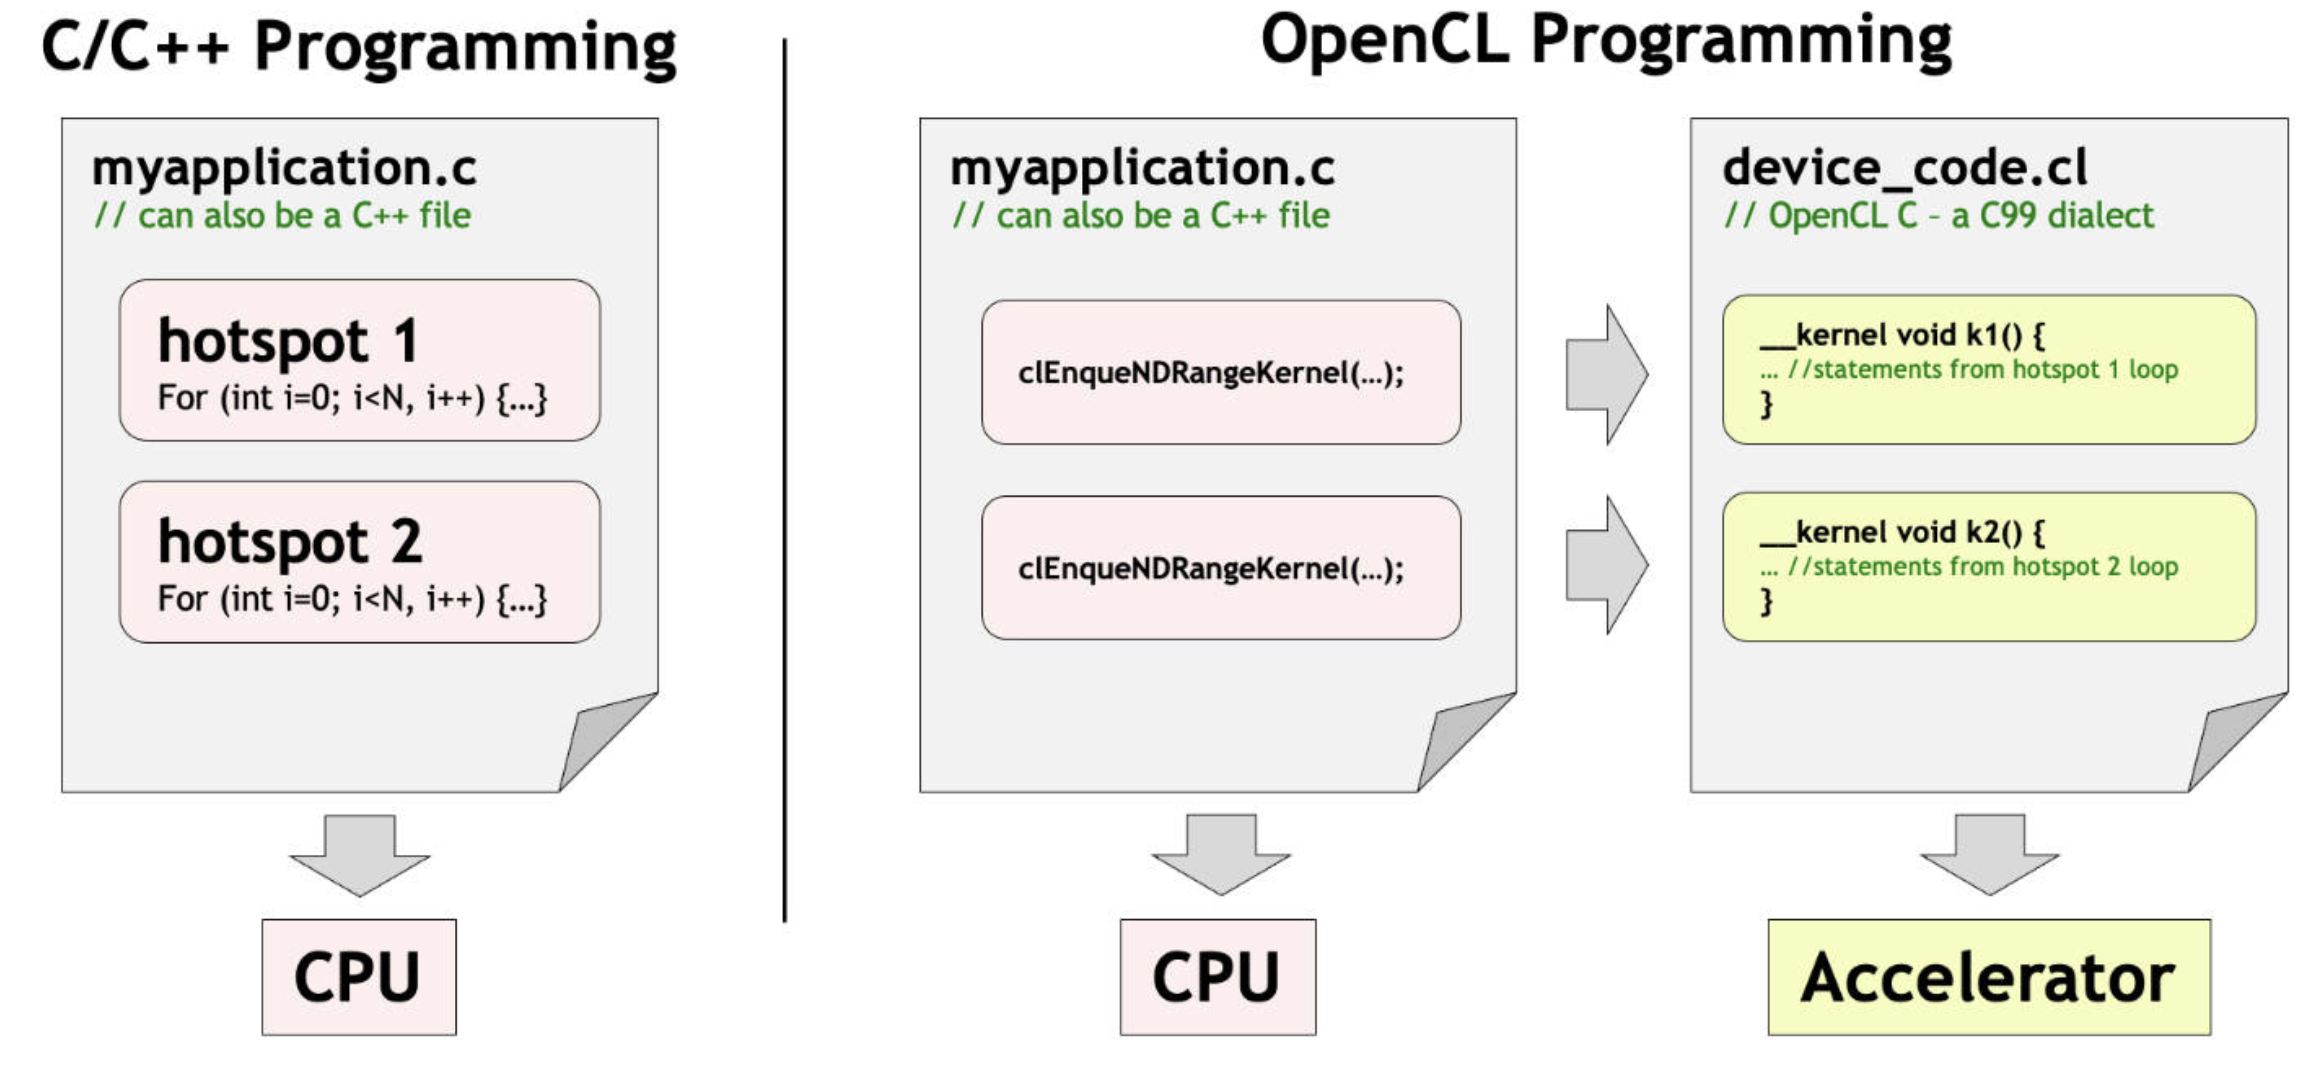
\includegraphics[scale=0.3]{images/Capitolo2/5_im.png}
    \caption{Traditional vs OpenCL programming paradigm}
    \label{funzionamentoOpenCL}
\end{figure}

\clearpage

\section{C++/C}
\label{C++/C}
I linguaggi di programmazione C e C++ sono due dei linguaggi più influenti e più utilizzati nella storia dell'informatica. Sono noti per la loro potenza, versatilità e velocità e sono utilizzati in una grande varietà di applicazioni, dai sistemi operativi al mondo del software per applicazioni generali. 

\vspace{0,3cm}
\vspace{0,3cm}

\noindent Di seguito un'introduzione a entrambi:

\vspace{0,3cm}
\noindent \textbf{Linguaggio C}:
\begin{itemize}
    \item È stato sviluppato negli anni 70 da Dennis Ritchie, ed è stato uno dei primi linguaggi ad alto livello della storia dell'informatica.
    \item È noto per la sua semplicità ed efficienza nell'accesso diretto alla memoria, ed è apprezzato per la possibilità di scrivere codice altamente ottimizzato.
    \item È ampiamente utilizzato per lo sviluppo di applicazioni embedded, sistemi operativi, compilatori e molte altre applicazioni a basso livello.
\end{itemize}

\vspace{0,3cm}
\noindent \textbf{Linguaggio C++}:
\begin{itemize}
    \item C++ è una versione estesa di C sviluppata negli anni '80 da Bjarne Stroustrup, tra le varie feature che aggiunge, c'è il concetto di programmazione orientata agli oggetti (OOP), il quale consente la creazione di software più strutturato e modulare rispetto al linguaggio C.
    \item È ampiamente utilizzato nell'industria del software, nei videogiochi, nella elaborazione di immagini e molto altro.
    \item Dispone di una libreria standard che presenta molti strumenti per lo sviluppo software. 

\end{itemize}

\vspace{0,3cm}
\vspace{0,3cm}

\noindent Entrambi sono linguaggi popolari, ma la scelta tra i due spesso dipende sia dall'applicazione specifica che dalle preferenze personali.
Tutti e due offrono un grado alto di controllo sulla macchina, ma C++ aggiunge il paradigma ad oggetti e una sintassi diversa per affrontare problemi complessi in modo più efficiente.

\vspace{0,3cm}

\noindent Abbiamo scelto di usare i linguaggi C e C++ per due motivi, in primo luogo perché rientrano tra la lista di linguaggi supportati dall'ambiente Vitis e dal framework OpenCL, inoltre la mia familiarità con questi ha facilitato lo sviluppo del progetto.



